\chapter{Hybrid Model Persistence}
\label{ch:hybrid_model_persistence}
Change-based persistence has the potential to support faster and more accurate model comparison, merging, as well as a range of analytics activities. However, reconstructing the state of a model by replaying its editing history every time the model needs to be queried or modified can get increasingly expensive as the model grows in size. In this work, we integrate change-based and state-based persistence mechanisms in a hybrid model persistence approach that delivers the best of both worlds. In this paper, we present the design of our hybrid model persistence approach and report on its impact on time and memory footprint for model loading, saving, and storage space usage.

\vspace{-20pt}
\section{Introduction}
\label{sec:introduction}
Change-based persistence (CBP) of models \cite{DBLP:conf/models/YohannisKP17} conforming to metamodelling architectures such as MOF/EMF \cite{omg2018mof,steinberg2008emf} comes with notable advantages over state-based persistence (SBP): it provides support for fast comparison and differencing of versions of the same model \cite{DBLP:conf/sde/LippeO92,DBLP:conf/caise/IgnatN05,DBLP:conf/edoc/KoegelHLHD10,koegel2010emfstore} -- which can also substantially speed up incremental model management activities, and enables novel model analytics activities (e.g. pattern detection in the editing history to understand how modellers use modelling languages and tools) \cite{DBLP:journals/entcs/RobbesL07}. However, CBP comes at the cost of ever-growing model files \cite{DBLP:conf/edoc/KoegelHLHD10,DBLP:journals/entcs/RobbesL07} since all changes (even deleting model elements) are recorded in an editing log, which naturally leads to longer loading times \cite{mens2002state}. In this work, we address the latter challenge by introducing the concept of hybrid persistence of models. In hybrid model persistence the change-based representation is augmented with a state-based representation (which may be derived from the change-based representation) of the latest state of the model which is used to speed up model loading and querying.

The paper is structured as follows. Section \ref{sec:change_and_state_based_model_persistence} introduces the concept of change-based model persistence and recent work on state-based model persistence. Sections \ref{sec:hybrid_model_persistence} and \ref{sec:implementation} present our approach to hybrid model persistence and its implementation. Section \ref{sec:evaluation} presents experimental results and evaluation. Section \ref{sec:related_work} provides an overview of related work, and Section \ref{sec:conlcusions_and_future_work} concludes with a discussion on directions for future work.

\vspace{-20pt}
\section{Change and State-based Model Persistence}
\label{sec:change_and_state_based_model_persistence}

\vspace{-10pt}
To explain the differences, benefits and drawbacks of CBP and SBP, consider a modelling activity on a UML model as presented Fig. \ref{fig:illustration_cbp}. The sub-figures \ref{fig:illustration_3} to \ref{fig:illustration_8} depict the evolution of a UML model at different time stamps. Classes are created and added/removed from \texttt{Package X}. In SBP, for each session, only the final state of the model is persisted (the state of previous session are overridden by the state of the latest session). Thus, to represent the final state of the UML model, only the information about \texttt{Package X} and \texttt{Class C} needs to be persisted, as presented in Listing \ref{lst:xmimodel2} (XMI format). In CBP, all the changes in the model are persisted. Thus, a list of all the events generated by the model editor is needed to represent the final state of the model.

\begin{figure}[ht]
    %    \begin{subfigure}[t]{0.245\linewidth}
    %        \centering
    %        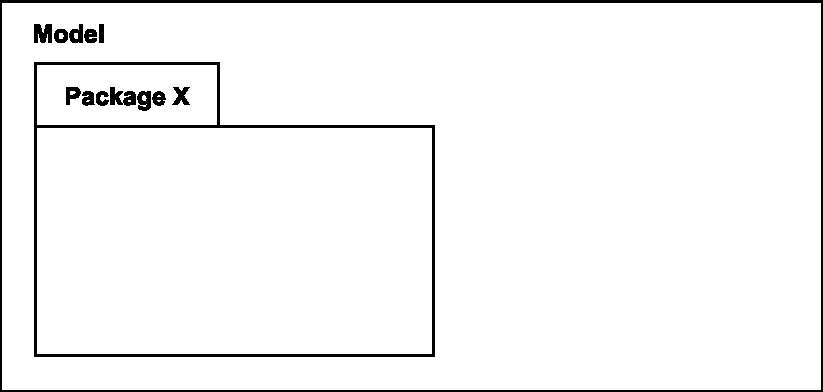
\includegraphics[width=\linewidth]{images/illustration_1}
    %        \caption{Initial state}
    %        \label{fig:illustration_1}
    %    \end{subfigure}
    %    \begin{subfigure}[t]{0.245\linewidth}
    %        \centering
    %        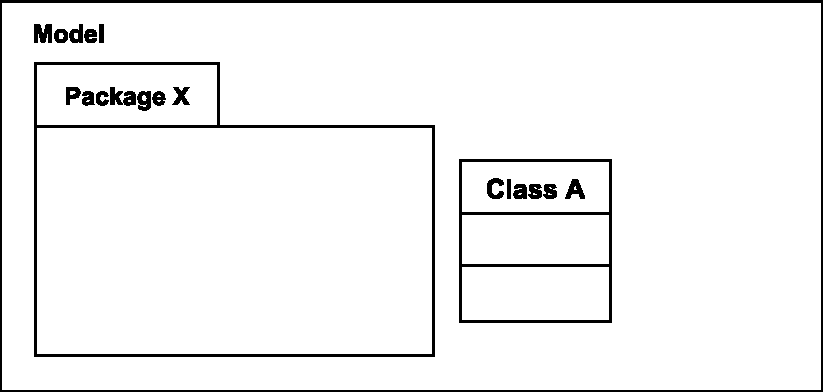
\includegraphics[width=\linewidth]{images/illustration_2}
    %        \caption{Time stamp 1}
    %        \label{fig:illustration_2}
    %    \end{subfigure}
    \begin{subfigure}[t]{0.329\linewidth}
        \centering
        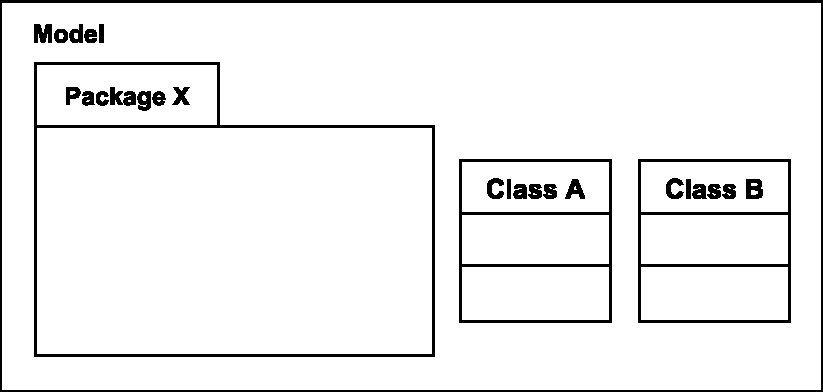
\includegraphics[width=\linewidth]{images/illustration_3}
        \caption{Time stamp 1}
        \label{fig:illustration_3}
    \end{subfigure}
    \begin{subfigure}[t]{0.329\linewidth}
        \centering
        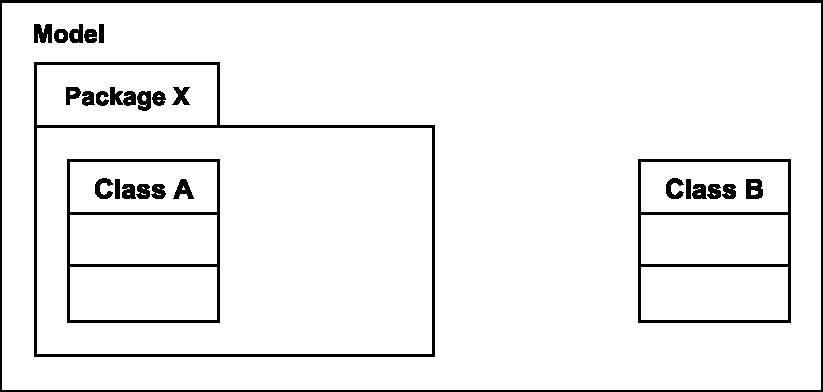
\includegraphics[width=\linewidth]{images/illustration_4}
        \caption{Time stamp 2}
        \label{fig:illustration_4}
    \end{subfigure}
    \begin{subfigure}[t]{0.329\linewidth}
        \centering
        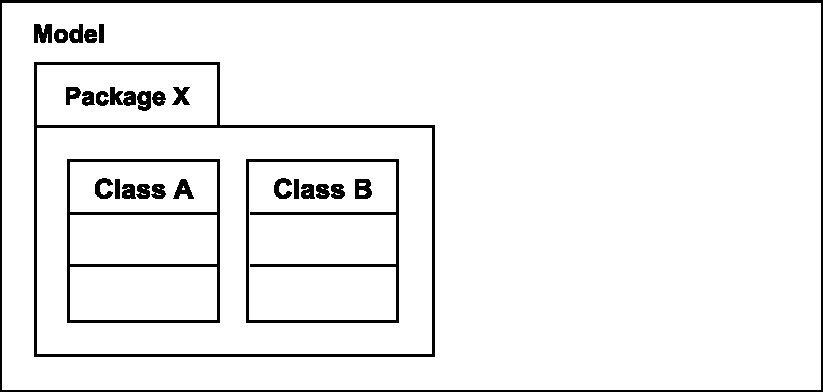
\includegraphics[width=\linewidth]{images/illustration_5}
        \caption{Time stamp 3}
        \label{fig:illustration_5}
    \end{subfigure}
    \hfill
    \begin{subfigure}[t]{0.329\linewidth}
        \centering
        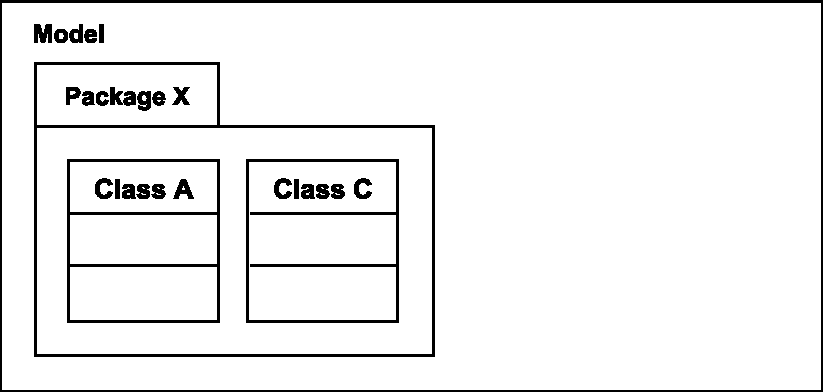
\includegraphics[width=\linewidth]{images/illustration_6}
        \caption{Time stamp 4}
        \label{fig:illustration_6}
    \end{subfigure}
    \begin{subfigure}[t]{0.329\linewidth}
        \centering
        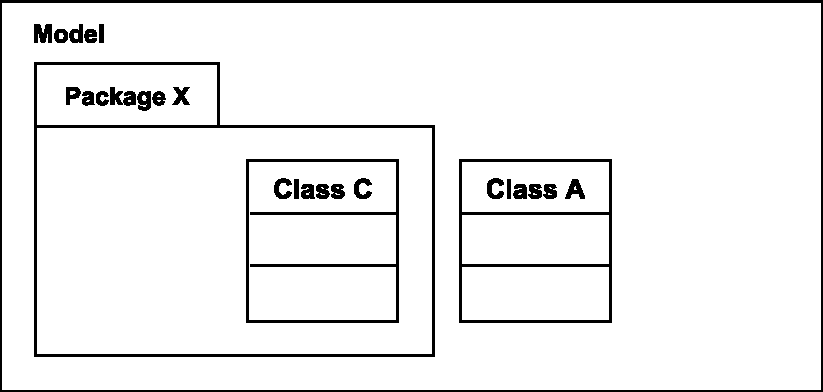
\includegraphics[width=\linewidth]{images/illustration_7}
        \caption{Time stamp 5}
        \label{fig:illustration_7}
    \end{subfigure}
    \begin{subfigure}[t]{0.329\linewidth}
        \centering
        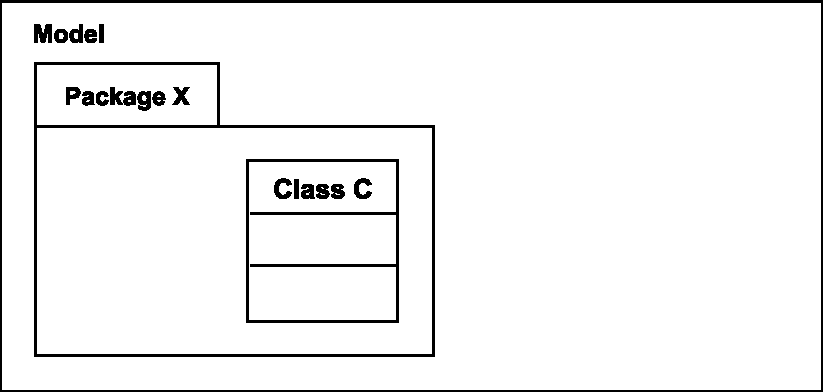
\includegraphics[width=\linewidth]{images/illustration_8}
        \caption{Time stamp 6}
        \label{fig:illustration_8}
    \end{subfigure}
    
    \caption{The states of the example model after certain changes and their corresponding lines in Listing \ref{lst:cbpmodel}.}
    \label{fig:illustration_cbp}
\end{figure}

A session depicts a set of changes made between $save$ events, i.e. a session comprises all the changes that happened since the last time that the model was persisted. The CBP representation is shown in Listing \ref{lst:cbpmodel}\footnote{We use a natural language pseudo-code for CBP, introduced in \cite{DBLP:conf/models/YohannisKP17,yohannis2018towards}}. Lines 1-7 represent the initial state (Fig. \ref{fig:illustration_3}), followed by lines 8 (Fig. \ref{fig:illustration_4}), 9 (Fig. \ref{fig:illustration_5}), 11 (Fig. \ref{fig:illustration_6}), 12 (Fig. \ref{fig:illustration_7}), and 13 (Fig. \ref{fig:illustration_8}). 

Table \ref{table:persistence_comparsion} summarises the benefits (+) and drawbacks (-) of change and state-based model persistence. To load an SBP model, only the elements that exist in the final state need to be loaded into memory. To load a CBP model, all the events that lead to the final state must be replayed to load the model in memory. Loading times for SBP models are proportional to the size of the model. Loading times for CBP models are proportional to the number of events. As a result, loading times of CBP models will always increase over time and are considerably longer than for SBP \cite{yohannis2018towards,mens2002state}. 

To store an SBP model, all the elements that exist in the final state must be persisted. To save a CBP, only the change events in the last session need to be persisted. Storing times of SBP models are proportional to the size of the model. Storing times of CBP models are proportional to the number of events in a session. As a result, storing times of CBP models can be considerably shorter than for SBP models \cite{yohannis2018towards}. Comparing and finding the differences between two versions of a state-based model is expensive \cite{Kolovos:2009:DMM:1564596.1564641} ($O(N^2)$ in the general case) which affects the efficiency of change visualisation and comprehension, and has a substantial impact on downstream activities such as incremental model transformation \cite{DBLP:conf/ecmdafa/OgunyomiRK15} and validation.

\vspace{-15pt}
\begin{minipage}[t]{0.59\linewidth}
    \begin{lstlisting}[style=xmi,caption={The UML2 model of the example model in Fig. \ref{fig:illustration_cbp}.},label=lst:xmimodel2]
    <uml:Package xmi:id="1" name="X">
    <packagedElement xsi:type="uml:Class" xmi:id="3" name="C"/>
    </uml:Package>
    \end{lstlisting}
    
    \centering
    \captionof{table}{Comparison of model persistence approaches.}
    \label{table:persistence_comparsion}
    \begin{small}
        \begin{tabular}{ c c c c }
            \hline 
            \textbf{Dimensions} & \textbf{Change-based} & \textbf{State-based} \\
            \hline 
            Load Time & $-$ & $+$ \\
            Save Time & $+$ & $-$ \\
            Comparison Time & $+$ & $-$ \\
            Storage Space & $-$ & $+$ \\
            \hline 
        \end{tabular}
    \end{small}
\end{minipage}
\hfill
\begin{minipage}[t]{0.39\linewidth}
    \begin{lstlisting}[style=eol,caption={The textual CBP for producing state-based model in List. \ref{lst:xmimodel2}. Its visual illustration is in Fig. \ref{fig:illustration_cbp}.},label=lst:cbpmodel]
    session 1
    create p1 type Package
    set p1.name to "X" 
    create c1 type Class
    set c1.name to "A"
    create c2 type Class
    set c2.name to "B"
    add c1 to p1.packagedElement 
    add c2 to p1.packagedElement
    session 2
    set c2.name to "C"
    remove c1 from p1.children 
    delete c1
    \end{lstlisting}
\end{minipage}

By contrast, in CBP, changes are first-class entities in the persisted model file and as such, model comparison and differencing is relatively inexpensive. The main downsides of CBP are it's model file sizes \cite{DBLP:journals/entcs/RobbesL07,DBLP:conf/edoc/KoegelHLHD10} and ever-increasing loading times \cite{mens2002state}. Loading times can be reduced by around 50\% by processing the changelog, detecting, memorising and subsequently ignoring change events that have no impact to the final state of the model. The loading times are still substantially longer -- more than 6.4 times slower and even longer as the persisted changes increase -- than loading times for state-based approaches \cite{yohannis2018towards}. 

\vspace{-15pt}
\section{Hybrid Model Persistence}
\label{sec:hybrid_model_persistence}

\vspace{-15pt}
To achieve the best of both worlds we introduce a hybrid model persistence approach which combines change-based and state-based model persistence, to work together side-by-side. An overview of the proposed approach is illustrated in Fig. \ref{fig:hybrid_persistence}. In the proposed approach a \textit{hybrid} model is stored in two representations at the same time: a change-based (e.g. using CBP) and a state-based representation (e.g. using XMI or a database-backed approach such as NeoEMF). The change-based representation is perceived as the main representation of a model, while the state-based representation can be fully derived from the change-based representation.

\textbf{Loading a hybrid model.} Models are loaded into in-memory object graphs that clients (e.g. editors, transformations) can then interact with\footnote{Depending on the state persistence mechanism, the object graph may be loaded in its entirety at startup (e.g. XMI) or loaded progressively, in a lazy manner (e.g. NeoEMF/CDO)}. In the proposed hybrid approach, if the state-based counterpart already exists, the in-memory object graph is populated from it; otherwise, it is populated by replaying the complete editing history recorded in the change-based representation.

\textbf{Changing a hybrid model.} When an element in a loaded model is created, modified or deleted, the change is applied to the in-memory object graph and is also recorded in an in-memory list of changes (\textit{Editing session changes} in Fig 2). We use the term \emph{editing session} for the period between loading a model and saving back to disk. 

\textbf{Saving a hybrid model.} The current version of the in-memory object graph is stored in the preferred state-based representation. The list of changes recorded in the current editing session (with optional processing, as described above) is appended to the change-based representation.

\textbf{Versioning a hybrid model.} Since the state-based representation is fully derived from the change-based representation, if a model needs to be versioned (e.g. in a Git repository), only the change-based representation needs to be stored. The first time it is loaded after being checked out/cloned, the state-based representation is computed and persisted locally and is used in subsequent model loading steps.

\textbf{Comparing hybrid models.} To compare two hybrid models\footnote{The work of the hybrid model comparison is still in the preliminary stage and out of the scope of this paper.}, their change-based representations are used: this is much more efficient than state-based comparison. 
%as demonstrated in Section \ref{sec:change_detection}.

\begin{figure}[t]
    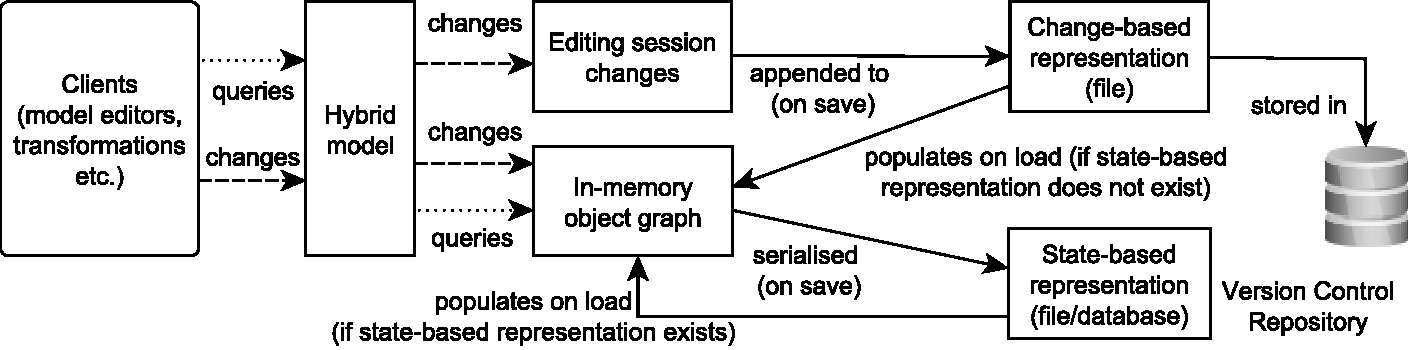
\includegraphics[width=\linewidth]{images/hybrid_persistence}
    \captionof{figure}{The mechanism of hybrid model persistence.}
    \label{fig:hybrid_persistence}
\end{figure}

\vspace{-15pt}
\section{Implementation}
\label{sec:implementation}

\vspace{-10pt}
We have implemented the proposed hybrid model persistence approach in a prototype\footnote{The prototype is available under \url{https://github.com/epsilonlabs/emf-cbp}.} on top of the Eclipse Modeling Framework (EMF) \cite{steinberg2008emf}. The prototype makes use of an existing implementation of change-based model persistence, the Epsilon CBP \cite{DBLP:conf/models/YohannisKP17}, augmented with two state-based persistence implementations: NeoEMF \cite{daniel2016neoemf} and XMI \cite{omg2018xmi}.

XMI has been selected as a standard state-based model persistence format (natively supported by EMF), and NeoEMF as a best-of-breed representative of database-backed state-based model persistence frameworks. The core components of the prototype are presented in Fig. \ref{fig:class_diagram}. 

\vspace{-15pt}
\begin{figure}[ht]
    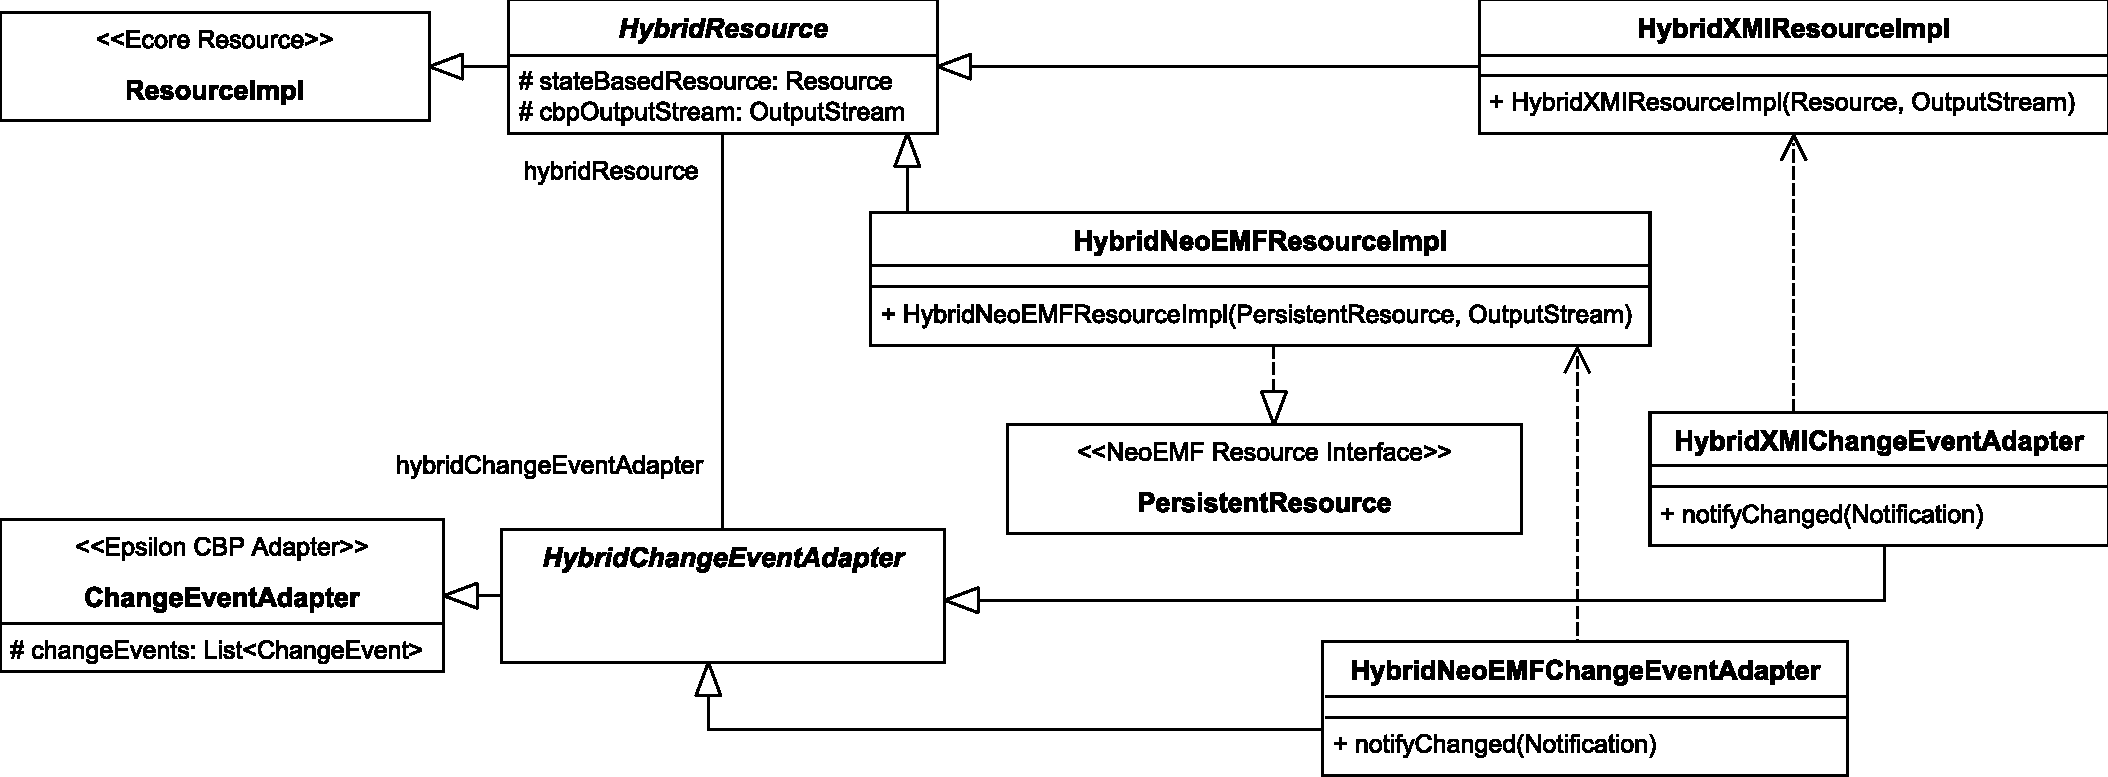
\includegraphics[width=\linewidth]{images/class_diagram}
    \captionof{figure}{Class diagram showing the core components of the hybrid model persistence implementation.}
    \label{fig:class_diagram}
\end{figure}

\vspace{-15pt}
The Epsilon CBP provides a \textsf{ChangeEventAdapter} class \cite{DBLP:conf/models/YohannisKP17} that extends from Ecore's \textsf{EContentAdapter} adapter class%\cite{eclipse2018eContentAdapter}
. This class collects changes made to the in-memory object graph of an EMF model in the form of a list of events \textsf{changeEvents}. Based on this class, we derived an adapter class, \textsf{HybridChangeEventAdapter}, for the hybrid model persistence implementation. It is an abstract class so that it can be further derived to create different implementations of adapter classes for different types of state-based persistence. The \textsf{HybridNeoEMFChangeEventAdapater} is the adapter class for NeoEMF, and the \textsf{HybridXMIChangeEventAdapater} for XMI. These classes override \textsf{notifyChanged}(\textsf{Notification}) in the \textsf{ChangeEventAdapter} class, to handle events that are specific to NeoEMF and XMI, respectively.

We also created a resource class for hybrid persistence, \textsf{HybridResource} (a resource class is a class dedicated to interacting with a persistence, e.g. save, load, get contents), derived from the Ecore's \textsf{ResourceImpl}%\cite{eclipse2018resourceImpl}
. The class is again abstract so that it can be realised in different resource implementation classes for different state-based persistence. The \textsf{HybridResource} class contains the \textsf{stateBasedResource} field which is used to refer to a state-based persistence that is being used, and the \textsf{cbpOutputStream} field that refers to an \textsf{OutputStream} (e.g. file, in-memory) as the representation of the CBP for saving changes. \textsf{HybridResource} has an association with \textsf{HybridChangeEventAdapater}, so that the former can access the events collected by the latter, and the latter can also use facilities provided by the former (e.g. getting the identity of an element in the resource; saving changes to a change-based model representation).

The resource implementation classes for NeoEMF and XMI are \textsf{HybridNeoEMFResourceImpl} and \textsf{HybridXMIResourceImpl} respectively. \textsf{HybridNeoEMFResourceImpl} also implements the NeoEMF's \textsf{PersistenceResource} interface %\cite{atlanmod2018persistentResource}
so that specific NeoEMF's methods can be used (e.g. \textsf{close}(), to close a connection with a backend database).


%\vspace{-15pt}
%\subsection{Known Limitations}
%
%\vspace{-10pt}
%Our prototype supports all the core constructs of Ecore, including classes, inheritance, single or multi-valued attributes and references, datatypes and containment. It also supports session-based changes to models that are atomic editor events, such as creating and deleting an object, setting and unsetting a feature. 
%
%With regard to notable limitations, the hybrid model persistence can only support single-file models: fragmented across multiple files and cross-model references models persisted in more than one file or backend. Secondly, an assumption is made that the two underpinning representations (change-based and state-based) are always consistent with each other, i.e. that they are always modified as an indivisible unit.

\vspace{-15pt}
\section{Evaluation}
\label{sec:evaluation}

\vspace{-10pt}
In this section, we compare hybrid model persistence (Epsilon CBP with each of NeoEMF and XMI) vs state-based persistence (NeoEMF or XMI only) on storage space usage, loading and saving time and memory footprint, and demonstrate that hybrid model persistence can still perform fast model loading and saving. 

%\vspace{-20pt}
%\begin{table}[ht]
%    \centering
%    \begin{footnotesize}
%        \caption{Space usage for the Epsilon and BPMN2 projects, and the Wikipedia's United States article.}
%        \label{table:space_usage}
%        \begin{tabular}{| c | c  c  c | c c c | c c c |}
%            \hline 
%            \textbf{Case} & \multicolumn{3}{c|}{\textbf{Epsilon}} & \multicolumn{3}{c|}{\textbf{BPMN2}} & \multicolumn{3}{ c |}{\textbf{Wikipedia}}\\
%            \hline
%            \makecell{Generated\\From} & \multicolumn{3}{c|}{940 commits} & \multicolumn{3}{c|}{192 commits} & \multicolumn{3}{ c |}{10,187 versions}\\
%            \hline
%            Type & XMI & NeoEMF & CBP & XMI & NeoEMF & CBP & XMI & NeoEMF & CBP \\
%            \hline
%            \makecell{Element\\Count} & 88,020 & 88,020 & --- & 62,062 & 62,062 & --- & 13,112 & 13,112 & --- \\
%            \hline
%            \makecell{Event\\Count} & --- & --- & 4.3 m & --- & --- &  1.2 m & --- & --- & 62.3 m \\
%            \hline
%            \hline
%            \makecell{Space\\Size} & \makecell{9.44\\MBs} & \makecell{188\\MBs} & \makecell{406\\MBs} & \makecell{6.55\\MBs} & \makecell{134\\MBs} & \makecell{109\\MBs} & \makecell{1.28\\MBs} & \makecell{31.8\\MBs} & \makecell{5.85\\GBs} \\
%            \hline
%            \makecell{Average\\Space\\Size} & \makecell{112\\bytes/\\element} & \makecell{2\\KBs/\\element}  & \makecell{98 \\bytes/\\event} & \makecell{110\\bytes/\\element} & \makecell{2\\KBs/\\element} & \makecell{92\\bytes/\\event} & \makecell{102\\bytes/\\element} & \makecell{2\\KBs/\\element} & \makecell{98\\bytes/\\event} \\
%            \hline 
%        \end{tabular}
%        \justify
%        m = million events, MB = Megabytes, KB = Kilobytes
%    \end{footnotesize}
%\end{table}

The evaluation was performed on Intel\textsuperscript{\textregistered} Core\textsuperscript{TM} i7-6500U CPU @ 2.50GHz 2.59GHz, 12GB RAM, and the Java\textsuperscript{TM} SE Runtime Environment (build 1.8.0 \textunderscore162-b12). For the evaluation, we used models reverse-engineered from the Java source code of the Epsilon \cite{eclipse2017epsilon,eclipse2018epsilongit} and BPMN2 \cite{eclipse2017bpmn2} projects. For state-based representation of the models, we used the MoDisco tool \cite{DBLP:journals/infsof/BruneliereCDM14} to generate XMI-based UML2 \cite{eclipse2017uml2} models that reflect the classes, fields, and operation signatures of the source code of the project and then imported the generated models into NeoEMF. We also derived MoDiscoXML models \cite{eclipse2018modiscoxml} from the Wikipedia article on the United States \cite{wikipedia2018us}. We then used reverse-engineering to generate a CBP for each project based on the differences between consecutive versions of the models.
%Reverse-engineering a state-based representation of a model is trivial; the change-based representing is more challenging. Here, a change-based representation was derived from the diffs identified from the subsequent versions of the Java source code committed on its Git repository. The change-based representation was derived by comparing an initially-empty running model to the generated models sequentially, ordered by their versions. All identified differences were then reconciled by performing a one-way merge to the running model. All changes made to the running model during the merging process were captured and persisted into a CBP file. The comparison and merging were performed using EMF Compare \cite{eclipse2017compare}. This procedure follows the procedure performed in \cite{yohannis2018towards}. 

\vspace{-20pt}
\begin{table}[ht]
    \centering
    \begin{footnotesize}
        \caption{Space usage for the Epsilon and BPMN2 projects, 
            and the Wikipedia's United States article.}
        \label{table:space_usage}
        \begin{tabular}{| c | c  c  c | c  c  c | c c c |}
            \hline 
            \textbf{Case} & \multicolumn{3}{c|}{\textbf{Epsilon}} & \multicolumn{3}{c|}{\textbf{BPMN2}} & \multicolumn{3}{ c |}{\textbf{Wikipedia}} \\
            \hline
            \makecell{Generated\\From} & \multicolumn{3}{c|}{940 commits} & \multicolumn{3}{c|}{192 commits} & \multicolumn{3}{ c |}{10,187 versions}\\
            \hline
            Type & XMI & NeoEMF & CBP & XMI & NeoEMF & CBP & XMI & NeoEMF & CBP \\
            \hline
            \makecell{Element\\Count} & 88,020 & 88,020 & --- & 62,062 & 62,062 & --- & 13,112 & 13,112 & --- \\
            \hline
            \makecell{Event\\Count} & --- & --- & 4.3 m & --- & --- & 1.2 m & --- & --- & 62.3 m \\
            \hline
            \hline
            \makecell{Space\\Size} & \makecell{9.44\\MBs} & \makecell{188\\MBs} & \makecell{406\\MBs} & 
            \makecell{6.55\\MBs} & \makecell{134\\MBs} & \makecell{109\\MBs} &
            \makecell{1.28\\MBs} & \makecell{31.8\\MBs} & \makecell{5.85\\GBs} \\
            \hline
            \makecell{Average\\Space\\Size} & \makecell{112\\bytes/\\element} & \makecell{2\\KBs/\\element}  & \makecell{98\\bytes\\/event} & 
            \makecell{110\\bytes/\\element} & \makecell{2\\KBs/\\element}  & \makecell{92\\bytes\\/event} &  
            \makecell{102\\bytes/\\element} & \makecell{2\\KBs/\\element} & \makecell{98\\bytes\\/event}  \\
            \hline 
        \end{tabular}
        \justify
        m = million events, MB = Megabytes, KB = Kilobytes
    \end{footnotesize}
\end{table}

\vspace{-25pt}
\subsection{Storage Space Usage}
\label{sec:storage_space_usage}

\vspace{-5pt}
For the Epsilon project, we have successfully generated a CBP from version 1 up to version 940 and also CBPs for the BPMN2 project and Wikipedia article up to version number 192 and 10,187 respectively. The details (element count, event count, space size, and average space size per element or event) of their models, when persisted in XMI, NeoEMF, and CBP are shown in Table \ref{table:space_usage}. The last row of the table derives an average space usage per element (for the SBPs) or event (for the CBP). We can estimate the storage space usage for a hybrid model persistence to be the combination of CBP and the appropriate SBP space usage.


\vspace{-20pt}
\begin{table}[ht]
    \centering
    \begin{footnotesize}
        \caption{The comparison on time and memory footprint for loading and saving models of the hybrid and state-based-only persistence.}
        \label{table:time_memory_footprint}
        \begin{tabular}{ | c | c | c | c | c | c | c | c | c | }
            \hline
            \multirow{2}{*}{\textbf{Dimension}} & \multirow{2}{*}{\textbf{Case}} & \multirow{2}{*}{\textbf{Backend}} & \multicolumn{2}{c|}{\textbf{Hybrid}} & \multicolumn{2}{c|}{\textbf{State-based}} & \multicolumn{2}{c|}{\textbf{Significance}} \\
            \hhline{~~~------}
            & & & $mean$ & $sd$ & $mean$ & $sd$ &  $W$ & $p$-$value$ \\
            \hline
            %----------------
            \multirow{4}{*}{\makecell{Loading\\Time}} & \multirow{2}{*}{Epsilon} & NeoEMF & 0.292 & 0.061 & 0.279 & 0.023 & 258 & \textbf{0.72}\\ 
            \hhline{~~-------}
            & & XMI & 0.317 & 0.006 & 0.270 & 0.018 & 26 & $<$ 0.05 \\
            \hhline{~--------}
            &\multirow{2}{*}{BPMN2} & NeoEMF & 0.308 & 0.071 &0.286 & 0.025 & 230 & \textbf{0.79}\\ 
            \hhline{~~-------}
            & & XMI & 0.212 & 0.016 & 0.179 & 0.016 & 37 & $<$ 0.05 \\
            \hhline{~--------}
            &\multirow{2}{*}{Wikipedia}  & NeoEMF & 0.262 & 0.048 & 0.273 & 0.062 & 250 & \textbf{0.86}\\ 
            \hhline{~~-------}
            & & XMI & 0.045 & 0.001 & 0.040 & 0.001 & 0 & $<$ 0.05 \\
            \hline
            \hline
            %--------------------
            
            \multirow{4}{*}{\makecell{Saving\\Time}} & \multirow{2}{*}{Epsilon} & NeoEMF & 0.0892 & 0.0421 & 0.0829 & 0.0494 & 216 & \textbf{0.55}\\ 
            \hhline{~~-------}
            & & XMI & 0.411 & 0.023 & 0.397 & 0.015 & 78 & $<$ 0.05 \\
            \hhline{~--------}
            &\multirow{2}{*}{BPMN2} & NeoEMF & 0.0777 & 0.0424 & 0.0775 & 0.0452 & 213 & \textbf{0.51}\\ 
            \hhline{~~-------}
            & & XMI & 0.33 & 0.007 & 0.28 & 008 & 0 & $<$ 0.05 \\
            \hhline{~--------}
            &\multirow{2}{*}{Wikipedia} & NeoEMF & 0.135 & 0.048 & 0.120 & 0.024 & 218 & \textbf{0.59}\\ 
            \hhline{~~-------}
            & & XMI & 0.024 & 0.048 & 0.020 & 0.002 & 42 & $<$ 0.05 \\
            \hline
            \hline
            %--------------------
            
            \multirow{4}{*}{\makecell{Loading\\Memory\\Footprint}} & \multirow{2}{*}{Epsilon} & NeoEMF & 38.601 & 0.878 & 10.014 & 1.088 & 0 & $<$ 0.05\\ 
            \hhline{~~-------}
            & & XMI & 10.72018 & 0.00022 & 10.72009 &0.00024 & 0 & $<$ 0.05 \\
            \hhline{~--------}
            &\multirow{2}{*}{BPMN2} & NeoEMF & 40.78 & 1.29 & 27.20 & 1.05 & 0 & $<$ 0.05\\ 
            \hhline{~~-------}
            & & XMI & 6.73367 & 1.29305 & 6.73367 & 0.00056 & 101 & $<$ 0.05 \\
            \hhline{~--------}
            &\multirow{2}{*}{Wikipedia}  & NeoEMF & 35.91 & 1.03 & 27.25 & 0.54 & 27.25 & \textbf{0.54}\\ 
            \hhline{~~-------}
            & & XMI & 8.4079 & 0.0008 & 8.0933 & 0.0009 & 0 & $<$ 0.05 \\
            \hline
            \hline
            %--------------------
            
            \multirow{4}{*}{\makecell{Saving\\Memory\\Footprint}} & \multirow{2}{*}{Epsilon} & NeoEMF & 2.64 & 1.29 & 2.61 & 0.78 & 283 & \textbf{0.34}\\ 
            \hhline{~~-------}
            & & XMI & 1.56355 & 0.0005 & 1.56326 & 0.0018 & 408 & $<$ 0.05 \\
            \hhline{~--------}
            &\multirow{2}{*}{BPMN2} & NeoEMF & 1.86 & 3.86 & 1.52 & 0.77 & 308 & \textbf{0.12}\\ 
            \hhline{~~-------}
            & & XMI & 0.8378 & 0.00361 & 0.8375 & 0.00362 & 58 & $<$ 0.05 \\
            \hhline{~--------}
            &\multirow{2}{*}{Wikipedia}  & NeoEMF & 1.32 & 1.51 & 0.97 & 0.76 & 189 & \textbf{0.22}\\ 
            \hhline{~~-------}
            & & XMI & 0.0010 & 0.00044 & 0.0005 & 0.00001 & 0 & $<$ 0.05\\ 
            \hline
            %--------------------
            
        \end{tabular}
        \justify
        The time is in seconds, and the memory footprint is in MBs.
    \end{footnotesize}
\end{table}

\vspace{-25pt}
\subsection{Time and Memory Footprint of Loading and Saving Models}
\label{sec:model_loading_time}

\vspace{-10pt}
We evaluated the performance of our hybrid persistence prototype against XMI and NeoEMF regarding time and memory footprint for loading and saving. We repeated our experiments 22 times for each dimension measured. Since the data were not normally distributed, we used the nonparametric Mann-Whitney U test \cite{doi:10.1002/9780470479216.corpsy0524} with a significance level of 5\%. 

As it can be noticed in Table \ref{table:time_memory_footprint}, all cases experience a slight slowdown on loading and saving time (hybrid approach's $mean$ $>$ state-based approach's $mean$). However, almost for all NeoEMF cases, the slowdown is not significant, which means that side-effect of the hybrid approach on loading and saving time is still acceptable. The hybrid approach also produces more memory footprint compared to the state-based-only approach. Nevertheless, considering the cost of main memory, this condition is acceptable in almost all real-world scenarios.




%\vspace{-20pt}
%\subsection{Change Detection}
%\label{sec:change_detection}
%
%\vspace{-10pt}
%We evaluated the contribution of CBP, as part of the hybrid model persistence, on model change detection. In this evaluation, we used four versions of the Epsilon project UML2 model: committed versions 8, 44, 181, and 388: details are in Table \ref{table:version_description}. As the scenario for the evaluation, we identify the elements in the older model (lower version number) that do not exist in the newer model (higher version number). Our dataset comprises the pairs, 008 and 044, 008 and 181, and 008 and 383.
%
%We used two methods to identify deleted elements. First, we iterated through events in the change-based representation of the pairs' hybrid-model representation (\emph{the hybrid method}). Second, we performed a model-to-model comparison between the two states of the paired versions (8 vs 44, 8 vs 181, 8 vs 388) using EMF Compare and selected diffs representing deleted elements (\emph{the state-based method}). We compared both methods on the time they required to identify all the deleted elements. We performed measurement 22 times for each pair and method to calculate the time. Fig. \ref{table:version_description} shows the result of the comparison. 
%
%%\begin{figure}[ht]
%%    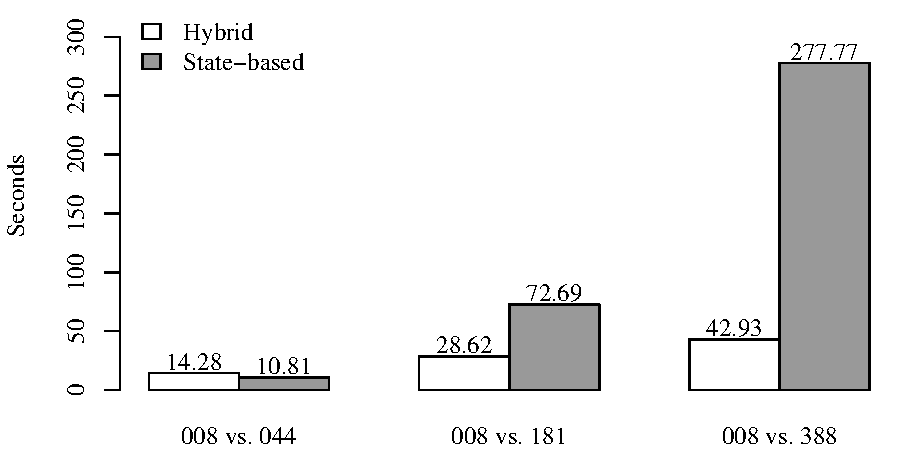
\includegraphics[width=\linewidth]{images/delete_detection_epsilon_average}
%%    \caption{The time required for hybrid and state-based methods on detecting older version's elements that do not exist in newer versions.}
%%    \label{fig:delete_detection_epsilon_average}
%%\end{figure}
%
%%\vspace{-40pt}
%As can be noticed in Table \ref{table:version_description}, identifying changed elements using the hybrid method is distinctly faster than using the state-based method (rows 3 and 4), except when the models being compared are small in size (row 1). Considering the increasing number of elements and events in Table \ref{table:version_description}, the change identification time of the hybrid method tends to grow linearly as the number of events increases, whereas the stated-based method tends to grow exponentially as the number of elements increases.
%
%\vspace{-20pt}
%\begin{table}[ht]
%    \centering
%    \caption{Description of version 8, 44, 181, and 388 of the Epsilon project's UML2 model, and delete detection time of hybrid and state-based methods.}
%    \label{table:version_description}
%    \begin{tabular}{| r | r | r | r | r || r | r | r | r | r |}
%        \hline 
%        \multirow{2}{*}{\textbf{\thead{Ver-\\sions}}} & \multirow{2}{*}{\textbf{\thead{Element\\Counts}}} & \multirow{2}{*}{\textbf{\thead{Delta\\Elements\\(from\\ver. 8)}}} & \multirow{2}{*}{\textbf{\thead{Event\\Counts}}} & \multirow{2}{*}{\textbf{\thead{Delta\\Events\\(from\\ver. 8)}}} & \multicolumn{4}{c|}{\textbf{\thead{Time for Delete Detection\\ in Seconds (from ver. 8)}}} \\
%        \hhline{~~~~~----}
%        & & & & & \multicolumn{2}{c|}{\textbf{\thead{Hybrid}}} & \multicolumn{2}{c|}{\textbf{\thead{State-based}}} \\
%        \hhline{~~~~~----}
%        & & & & & \textbf{\thead{\textit{mean}}}& \textbf{\thead{\textit{sd}}} &  \textbf{\thead{\textit{mean}}}& \textbf{\thead{\textit{sd}}} \\
%        \hline 
%        008	& 25,993 & 0	& 90,888 & 0 & --- & --- & --- & --- \\
%        044	& 31,240 & 5,247	& 166,659 & 75,771 & 14.28 & 0.36 & 10.81 & 0.16  \\
%        181	& 34,196 & 8,203	& 250,073 & 159,185 & 28.62 & 0.17 & 72.69 & 1.28 \\
%        388	& 48,482 & 22,489 & 332,315 & 241,427 & 42.93 & 0.18 & 277.77 & 4.70 \\
%        \hline 
%    \end{tabular}
%    \justify
%\end{table}

%\subsection{Threats to Validity and Limitations}
%\label{sec:threats_to_validity_and_limitations}
%Since change-based model persistence is a relatively new concept, there are hardly any such models available in public repositories that we could reuse for evaluating our prototype. So far, we have only tested the hybrid model persistence approach on synthesised models which may not be representative of the characteristics of models created by people.

\vspace{-20pt}
\section{Discussion}
\label{sec:discussion}

\vspace{-10pt}
%The evaluation results for change detection, Section \ref{sec:change_detection}, show that model change detection in hybrid model persistence is substantially faster than state-based comparison. This is because elements and features that have been modified can be directly identified through the events recorded in its CBP representation without the need to compare the models element-by-element. 
The use of state-based persistence in hybrid model persistence enables faster model loading, as shown by the result of loading time evaluation in Section \ref{sec:model_loading_time}, without having to replay all the changes persisted in its CBP -- the main challenge for the change-based approach \cite{yohannis2018towards,mens2002state}. 
Hybrid model persistence performs slightly slower -- statistically significant for Hybrid XMI but insignificant for Hybrid NeoEMF -- compared to loading a state-based model. A slight slowdown also appears on model saving -- statistically significant for Hybrid XMI but insignificant for Hybrid NeoEMF (Section \ref{sec:model_loading_time}). The slowdown is because changes have to be persisted into two representations, state-based and change-based. 

The main drawback of hybrid model persistence is that it consumes more memory when loading and saving and storage space for persisting models compared to state-based representation only (Sections \ref{sec:model_loading_time} and \ref{sec:storage_space_usage}). However, considering the cost of main memory and storage, the trade-off can be acceptable in most real-world scenarios.

\vspace{-10pt}
\section{Related Work}
\label{sec:related_work}
%Change-based persistence approaches have been used widely in incremental model management engines (e.g. IncQuery \cite{DBLP:conf/ecmdafa/RathHV12}, ReactiveATL \cite{DBLP:conf/ecmdafa/OgunyomiRK15}) usually by harnessing the notification facilities provided by the underlying modelling framework (e.g. EMF). Such approaches have also been applied in other software \cite{DBLP:journals/entcs/RobbesL07}, databases \cite{DBLP:conf/sde/LippeO92}, hierarchical documents \cite{DBLP:conf/caise/IgnatN05}, model repositories and version control \cite{koegel2010emfstore}. The approach is faster for detecting changes \cite{DBLP:conf/edoc/KoegelHLHD10}, more accurate and carries semantic information (e.g. actors, objects, timestamps, and sequences involved in events) \cite{DBLP:journals/entcs/RobbesL07,DBLP:conf/sde/LippeO92,DBLP:conf/caise/IgnatN05,mens2002state}, faster and more accurate for comparison and merging \cite{DBLP:conf/sde/LippeO92,DBLP:conf/caise/IgnatN05,koegel2010emfstore}, and enable additional analytics activities \cite{DBLP:journals/entcs/RobbesL07}.

\vspace{-10pt}
There are several non-XMI approaches to state-based model persistence, using relational or NoSQL databases. For example, EMF Teneo \cite{eclipse2017teneo} persists EMF models in relational databases, while Morsa \cite{DBLP:conf/models/Espinazo-PaganCM11} and NeoEMF \cite{daniel2016neoemf} persist models in document and graph databases, respectively. None of these approaches provides built-in support for versioning and models are eventually stored in binary files/folders which are known to be a poor fit for text-oriented version control systems like Git and SVN. Connected Data Objects (CDO) \cite{eclipse2017cdo}, which provides support for database-backed model persistence, also provides collaboration facilities, but CDO adoption necessitates the use of a separate version control system (e.g. a Git repository for code and a CDO repository for models), which introduces fragmentation and administration challenges \cite{barmpis2014evaluation}. Similar challenges arise in relation to other model-specific version control systems such as EMFStore \cite{koegel2010emfstore}. %prefer this to the wording in the repository version!

\vspace{-10pt}
\section{Conclusions and Future Work}
\label{sec:conlcusions_and_future_work}

\vspace{-10pt}
In this paper, we have proposed a hybrid model persistence approach and evaluated its impact on time and memory footprint for model loading and saving, and storage space usage.
%, and detecting changes of versions of the same model. 
Based on the evaluation results, the hybrid model persistence provides benefits on model loading time 
%and change detection 
with an acceptable trade-off on memory footprint and storage space usage. 

Currently, we are still working on the hybrid model comparison (Section \ref{sec:hybrid_model_persistence} -- Comparing hybrid models). So far, the progress is promising. Based on our preliminary investigation, it can detect atomic changes of models faster than state-based model comparison, e.g. detecting elements that have been removed from older versions. In the future, we plan to evaluate hybrid model persistence on even larger models and perform experiments where software modellers are asked to construct change-based models. We also plan to develop a solution for the efficient merging of change-based and hybrid models. 
